%\documentclass[11pt,a4paper,runningheads]{llncs}
\documentclass[11pt,a4paper]{article}
%encoding
%--------------------------------------
\usepackage[T1]{fontenc}
\usepackage[utf8]{inputenc}
%--------------------------------------

%Portuguese-specific commands
%--------------------------------------
\usepackage[portuguese]{babel}
%--------------------------------------

%Hyphenation rules
%--------------------------------------
\usepackage{hyphenat}
\hyphenation{mate-mática recu-perar}
%--------------------------------------

\usepackage{graphicx}
\usepackage{comment}
\usepackage{pgfplots}
\usepackage{amsmath,amssymb,amsfonts}
\usepackage{algorithmic}
\usepackage{graphicx}
\usepackage{textcomp}
\usepackage{xcolor}
\usepackage{adjustbox}
\usepackage{float}


\begin{document}

\title{Fase 3 - Requisitos, Casos de Uso e Arquitetura}
\author{Pedro Carrega, nº49480 \and
Vasco Ferreira, nº49470 \and Ye Yang, nº 49521
}

%\institute{Departamento de Informática da Faculdade de Ciências da Universidade de Lisboa
%\email{\{fc49480,fc49470,fc49521\}@alunos.fc.ul.pt}}

\maketitle

\section{Motivação para Dataset e Serviços}

O dataset ecommerce foi escolhido pelo grupo devido ao grande número de eventos gerados e consequente informação produzida durante a utilização de uma loja de ecommerce. Informação esta que pode ser utilizada de diversas formas através de um grande número de variados serviços. Essa mesma informação poderá ser utilizada em vários contextos, sendo que escolhemos os seguintes 5 serviços que demonstram diferentes tipos de informação sobre o dataset:

\begin{itemize}
  \item api/products/listCategories: Fornece todas as diferentes categorias presentes nos dados
  \item api/products/popularBrands: Fornece a contagem de eventos associados a cada marca
  \item api/products/salesByBrand: Lista o numero de vendas de cada marca
  \item api/products/salePrice: Calcula o valor médio de venda de uma determinada marca
  \item api/events/ratio: Apresenta a distribuição relativa de cada tipo de evento, havendo os possíveis valores: view, cart e purchase
\end{itemize}

Os serviços foram escolhidos de forma a que consigam fazer diferentes tipos de operações sobre os dados, desde serviços mais específicos e por isso com menos carga na base de dados, a serviços mais abrangentes e consequente aumento de carga. Foram também escolhidos pois todos os serviços fornecem dados úteis para serem explorados no contexto de lojas de ecommerce.

\section{Diagrama de Casos de Uso}
\begin{figure}[H]
  \centering
    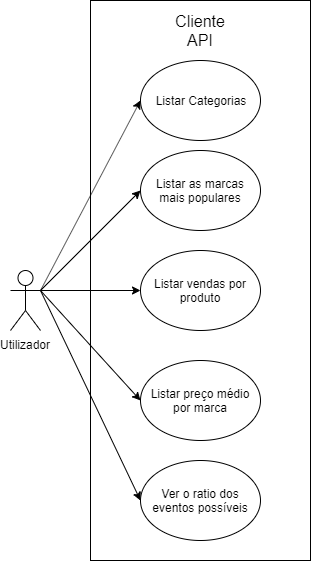
\includegraphics[scale=0.42]{Use_Cases.png}
  \caption{Diagrama de casos de uso}
\end{figure}

\section{Requisitos}

\begin{table}[H]
	\begin{center}
		\begin{tabular}{|p{3.5cm}|p{9.5cm}|}
		\hline
			\textbf{Requisitos\newline Não Funcionais} & \textbf{Descrição}\\ \hline
			Portabilidade & Implementação de servidor em NodeJS e cliente em HTML de modo a facilitar o processo de mudança de plataforma do serviço \\ \hline
			Legibilidade & A separação clara entre as camadas de apresentação, lógica de negócio e acesso à base de dados irá tornar o fluxo do sistema mais legível para os desenvolvedores \\ \hline
			Estabilidade & A distribuição do sistema por diversas máquinas virtuais, que poderão estar distribuídas por diferentes fornecedores cloud e em diferentes Data Centers permitem obter um sistema estável \\ \hline
			Elasticidade & O sistema deverá ser capaz de se adaptar à carga de trabalho através do provisionamento e desprovisionamento dos recursos de forma autónoma. Idealmente, de forma que em qualquer ponto do tempo, o sistema apenas utilize o número de máquinas necessárias de forma a corresponder à carga atual \\ \hline
			Escalabilidade & Capacidade do sistema lidar com o crescimento de carga de trabalho. Pode-se associar à capacidade de elasticidade do sistema \\ \hline
			Confiabilidade & Visto o sistema estar implementado na núvem, conseguimos garantir alta confiabilidade nos sistema, pois se um servidor no datacenter falhar, conseguimos facilmente migrar a VM para outro servidor funcional \\ \hline
	\end{tabular}
	\label{tab1}
	\end{center}
	\caption{Requisitos Não Funcionais}
\end{table}

\begin{table}[H]
	\begin{center}
		\begin{tabular}{|p{3.8cm}|p{8.2cm}|}
		\hline
			\textbf{Requisitos\newline Funcionais} & \textbf{Descrição}\\ \hline
			Listar\newline Categorias Disponíveis & Serviço que fornece aos clientes todas as categorias \\ \hline
			Visualizar\newline Popularidade das\newline Marcas & Serviço que fornece cada marca associada com a sua popularidade\\ \hline
			Visualizar\newline Número de Vendas\newline Individuais & Fornece o numero total de vendas de cada marca\\ \hline
			Visualizar\newline Preço Médio de Venda & Fornece o preço médio dos produtos vendidos de uma determinada marca \\ \hline
			Visualizar\newline Rácio de Tipo\newline de Eventos & Fornece a percentagem de cada tipo de evento \\ \hline
	\end{tabular}
	\label{tab2}
	\end{center}
	\caption{Requisitos Funcionais}
\end{table}

\section{Arquitetura da aplicação}
\begin{figure}[H]
  \centering
  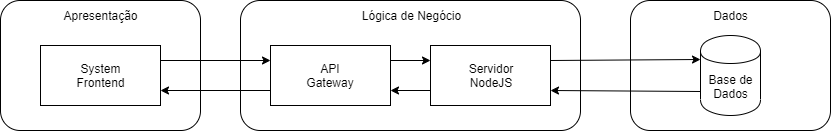
\includegraphics[scale=0.4]{App_arc.png}
  \caption{Arquitetura da aplicação}
\end{figure}

Após a definição da API com o Swagger na fase anterior, possibilitou a opção de exportar do API definido um Cliente (em Java) e um Servidor NodeJS.

\subsection{System Frontend}
O frontend irá dispor as funcionalidades anteriormente definidas. Pode ser extraído do ficheiro Swagger em formato HTML.
\newline

\subsection{API Gateway}
Este gateway irá ser encarregado de receber pedidos HTTP vindos do frontend e reencaminhá-los para o servidor NodeJS que tratará da lógica de negócio. Também irá encaminhar as respostas vindas do servidor para o frontend de modo disponibilizar os dados pretendidos.
\newline %removam isto se nao gostarem do espaço k adiciona


\subsection{Servidor NodeJS}
O servidor exportado do Swagger irá receber os pedidos a partir da API Gateway, e processá-los de acordo com a funcionalidade pretendida. A lógica de negócio é aqui tratada, realizando as queries necessárias para a base de dados. Ao receber os dados, processa-os de acordo com a funcionalidade, e encaminha o resultado para a gateway.
\newline %removam isto se nao gostarem do espaço k adiciona

\subsection{Base de dados}
A base de dados irá conter o conteúdo dos ficheiros .csv do nosso data set, que são acedidos pelo servidor de modo a poder efetuar as leituras necessárias para produzir uma resposta para o cliente. 
%\newpage
\section{Arquitetura técnica}
%Digam-me o que acham

%Não sei o que dizer da Portabilidade
Para garantir os requisitos não funcionais mencionados a cima devemos ter em atenção os serviços da cloud escolhidos, pois proporcionam vários aspetos fundamentais dos requisitos.
\newline

A utilização dos serviços disponibilizados pela AWS permite cumprir alguns dos requisitos não funcionais mencionados, nomeadamente a Escalabilidade e a Elasticidade. A implementação da API através da API Gateway permite que este serviço da cloud trate automaticamente da carga de pedidos HTTP recebida, não sendo necessário a criação de scripts especializados para distribuição de carga. A base de dados a ser implementada na Amazon DynamoDB também permite escalabilidade e também eficácia na resolução de queries, tratando da carga de queries automaticamente tal como os restantes serviços da cloud.
\newline

A Confiabilidade do sistema também é melhorada com a instalação em serviços na cloud, visto estas terem deteções automáticas de falhas de servidores, possibilitando a migração do sistema virtualizado para outro servidor funcional.
\newline

A Estabilidade é garantida nas várias ferramentas usadas na instalação do sistema. O API Gateway da AWS tratará automaticamente da carga de pedidos HTTP recebida, não sendo necessário a criação de scripts para mitigação de carga.
\newline

Já a Estabilidade é garantida devido a ter a Lógica de negócio distribuída por várias máquinas virtuais que cumprem a função de servidores.
\newline

Dado que o API é definido em Swagger, a implementação do cliente e servidor são facilmente traduzidos para uma outra linguagem exportável, garantindo a Portabilidade. Visto que a lógica de negócio vai ser implementada num servidor NodeJS, a maior parte do código desenvolvido poderá ser instalado noutra plataforma Cloud sem grandes mudanças, sendo as principais diferenças o acesso à base de dados da nova plataforma e a comunicação com a API Gateway. A camada de apresentação também não sofraria de mudanças de grau elevado, sendo que apenas a comunicação para a API Gateway mudaria.


\section{Lançamento em Kubernetes}
O scripts de deployment do sistema foram separados em 4 devido à necessidade dos clusters e node groups estarem ativos, antes de proceder aos próximos passos. Existe também uma secção de edição de ficheiro manual, o que fez a quebra entre o terceiro e o quarto script.

Antes da execução dos scripts é necessário verificar a existência dos seguintes repositórios, roles e policies e caso existam, precisam de ser \textbf{eliminados}:
\begin{enumerate}
	\item Repositórios com nomes \textit{products} e \textit{events}
	\item AWS Role com nome eksServiceRole
	\item AWS Policy com nome ALBIngressControllerIAMPolicyEcommerce
\end{enumerate}

Para a execução dos scripts são necessárias as seguintes ferramentas:
\begin{itemize}
	\item AWS CLI
	\item eksctl
	\item kubectl
\end{itemize}

A região a escolher para o lançamento poderá ser qualquer um, porém recomendamos a região eu-west-1. Esta região terá de ser a mesma nos argumentos de todos os scripts que requeiram a mesma.


\subsection{deploy1.sh}
O primeiro script de deployment recebe 3 argumentos na seguinte ordem:
\begin{enumerate}
	\item A região onde a Stack e o Cluster vão ser lançados (ex.: \textbf{eu-west-1})
	\item O nome da Stack que terá de ser único (nenhuma outra Stack na CloudFormation da conta pessoal poderá ter o mesmo nome) para o script funcionar corretamente (ex.:\textbf{ecommerce-stack})
	\item O nome do Cluster que também terá de ser único (ex.:\textbf{ecommerce-cluster})
\end{enumerate}

A criação da stack e do cluster irá demorar cerca de 10 a 20 minutos até ficarem ativos, após o qual poderemos proceder à execução do segundo script. O estado do script pode ser verificado com o seguinte comando:
\begin{itemize}
	\item \textit{aws eks describe-cluster --name CLUSTER\_NAME} , mudando CLUSTER\_NAME para o nome do cluster dado nos argumentos
\end{itemize}
A execução do segundo script só deve ser feita quando o estado do cluster estiver em \textbf{ACTIVE}.

\subsection{deploy2.sh}
O segundo script recebe os mesmos argumentos que o primeiro, todos na mesma ordem. Neste script vão ser criados os node groups e o pull das imagens dos serviços.

Para realizar o pull, irá ser pedido para inserir os credenciais IAM que dão acesso aos repositórios por nós criados. Estes credenciais encontram-se no ficheiro \textbf{credenciais.txt} juntamente com a região onde os repositórios se encontram.

No fim

\end{document}